\documentclass[12pt]{article}

\usepackage[letterpaper,margin=1in]{geometry}
\usepackage{mathptmx}
\usepackage{graphicx}
\usepackage{booktabs}
\usepackage{tabularx}
\usepackage{array}
\usepackage{float}
\usepackage[hidelinks]{hyperref}
\usepackage{caption}

\captionsetup{font=small,labelfont=bf}
\setlength{\parindent}{0pt}
\setlength{\parskip}{0.55em}
\renewcommand{\arraystretch}{1.08}
\graphicspath{{figures_accelergy_plugin/}}

\title{\vspace{-0.5in}Deadline-Constrained Systolic Array Design for Image Processing}
\author{Blake Wang and Yu Cheng Wu\\CSEN 318 High-Performance Computer Architecture and Systems, Spring 2026}
\date{}

\begin{document}
\maketitle

\section{Introduction}

\textbf{Motivation.} Real-time embedded vision systems process frames on a fixed schedule. A 30 FPS camera pipeline receives a new frame every 33.33 ms, so the accelerator does not need to be the fastest possible design. It needs to finish the full image-processing pipeline before the frame deadline while using as little energy as possible. This distinction matters because many accelerator studies report throughput or latency first, while an always-on edge camera also has a strict energy budget.

\textbf{Application boundary.} This project studies a grayscale image-processing front end:
\[
\text{input frame} \rightarrow \text{Gaussian blur} \rightarrow \text{Sobel edge detection} \rightarrow \text{edge frame}.
\]
The project models accelerator performance and energy for the two compute stages. It does not model camera capture, display, CPU orchestration, software scheduling overhead, image quality, or full-system idle power. Those parts are outside the boundary of this class project and are treated as system-level integration work rather than accelerator-kernel work.

\textbf{Objective.} The objective is to find the minimum-energy systolic array configuration that completes a full image frame before a target deadline. Each design is defined by array size, SRAM budget, external memory bandwidth, dataflow, Gaussian kernel size, image resolution, and frame deadline. For each design, the framework estimates full-frame latency, full-frame energy, average power at a target frame rate, energy-delay product, and deadline feasibility. The selection rule is to simulate tiled Gaussian and Sobel workloads, scale tile-level results to a full frame, convert compute and memory activity into Accelergy action counts, remove designs that miss the deadline, and select the minimum-energy feasible design.

\textbf{Literature and market context.} Systolic arrays are a standard architecture for regular matrix-style computation because processing elements can reuse operands while data moves through the array \cite{kung1982}. Modern vision and machine-learning accelerators use similar ideas because image filters and convolution layers can be expressed as matrix operations. SCALE-Sim provides a configurable cycle-level systolic-array simulator \cite{scalesim}, while Accelergy provides architecture-level energy estimation from component actions and energy reference tables \cite{accelergy}. The market motivation is embedded and edge vision, where power budgets matter as much as raw throughput. A camera service may target 24 FPS for video-like processing, 30 FPS for common real-time vision, or 60 FPS for smoother interactive systems. The experiment therefore treats the frame deadline as a first-class constraint instead of optimizing only for minimum latency.

\section{System Design and Implementation Details}

\textbf{Application scenario.} The modeled application is a grayscale camera front end. Each frame is first smoothed with Gaussian blur to reduce noise, then passed through Sobel edge detection to produce horizontal and vertical gradients. The Gaussian stage has variable compute intensity because the kernel sizes are swept across $3\times3$, $5\times5$, $7\times7$, and $11\times11$. Sobel always uses two $3\times3$ filters. The end-to-end modeled frame latency and energy are
\[
T_{\text{frame}} = T_{\text{gaussian}} + T_{\text{sobel}},
\quad
E_{\text{frame}} = E_{\text{gaussian}} + E_{\text{sobel}}.
\]
The output overhead in \path{configs/experiment.yaml} is set to 0 cycles. This is an explicit simplification so the project focuses on accelerator mapping and architecture tradeoffs for the two compute stages.

\textbf{Workload mapping.} The experiment is not a set of arbitrary GEMMs. Each image-filter tile is lowered into a GEMM-like workload because SCALE-Sim accepts matrix-style inputs. For one output pixel, a stencil filter is a dot product between a local image neighborhood and filter weights. For a whole output tile, these dot products become
\[
\text{output matrix} = \text{lowered image neighborhoods} \times \text{filter weights}.
\]
For Gaussian blur, $M$ is the number of output pixels in the tile, $N=1$ is the output channel count, and $K$ is the square of the Gaussian kernel size. For Sobel, $M$ is again the number of output pixels, $N=2$ for the horizontal and vertical gradient filters, and $K=9$ input values per $3\times3$ filter. These are skinny GEMMs because $N$ is only 1 or 2. That shape is important: a large systolic array can have poor utilization if the workload does not expose enough parallelism across matrix dimensions.

\begin{table}[H]
\centering
\small
\caption{Image-processing stages lowered to SCALE-Sim GEMM-style workloads.}
\begin{tabularx}{\textwidth}{l l l X}
\toprule
Stage & $M$ & $N$ & $K$ and modeled work \\
\midrule
Gaussian blur & Output pixels in tile & 1 & Kernel area; $9$, $25$, $49$, or $121$ MACs per output pixel. \\
Sobel edge detection & Output pixels in tile & 2 & $9$ input values for each of the $G_x$ and $G_y$ filters; $18$ MACs per output pixel. \\
\bottomrule
\end{tabularx}
\end{table}

\textbf{Tiled full-frame scaling.} Directly simulating every full frame for every design would be too slow. The framework simulates representative $128\times128$ output tiles and scales them to full frames. It handles full interior tiles, right-edge tiles, bottom-edge tiles, and corner tiles. Halo pixels are included in input traffic because convolution filters need neighboring pixels, but halo pixels do not produce additional output pixels. For each tile class, SCALE-Sim reports cycles, stalls, utilization, SRAM accesses, and DRAM accesses. The framework multiplies those values by the tile-class count and then sums Gaussian and Sobel to produce frame-level metrics.

\textbf{Tools and active pipeline.} The implementation uses Python scripts and a reusable \path{src/hpc_final} package for workload generation, tiling, parsing, aggregation, and plotting. SCALE-Sim estimates cycles, utilization, stalls, SRAM accesses, and DRAM accesses. Accelergy is used through the component-library/table-plug-in path to generate per-action energy values. Pandas and Matplotlib generate summary CSVs and figures, and Pytest covers config parsing, workload shapes, tiling, energy accounting, result aggregation, and SCALE-Sim I/O generation. The active pipeline is image-filter stage to GEMM topology, SCALE-Sim report, action counts, Accelergy ERT, and final energy and latency summaries. CACTI, Timeloop, Aladdin, RTL synthesis, and measured silicon power are not part of the final pipeline.

\textbf{Design space and assumptions.} The coarse sweep covers three resolutions: 720p, 1080p, and $2048\times2048$. It evaluates Gaussian kernels of $3\times3$, $5\times5$, $7\times7$, and $11\times11$; array sizes from $8\times8$ to $128\times128$; SRAM budgets of 256 KB, 1024 KB, and 4096 KB; bandwidths of 50 GB/s, 200 GB/s, and 800 GB/s; and weight-stationary, output-stationary, and input-stationary dataflows. A focused refinement sweep is added around the main 1080p real-time objective. It evaluates $32\times32$, $48\times48$, $64\times64$, $96\times96$, and $128\times128$ arrays; SRAM budgets from 256 KB to 4096 KB; 50 GB/s and 100 GB/s bandwidth; and weight-stationary plus input-stationary dataflows.

\textbf{Timing and energy model.} The clock is modeled as 1 GHz, so $\text{latency}_{ms}=\text{cycles}/10^9 \times 1000$. At 1 GHz, 60 FPS corresponds to 16.67 million cycles, 30 FPS to 33.33 million cycles, and 24 FPS to 41.67 million cycles. Changing the clock would linearly scale latency and deadline feasibility, but it would not change the counted MAC, SRAM, or DRAM actions for a fixed SCALE-Sim run. The energy model is dynamic action-count energy. It includes MAC actions and SRAM/DRAM read/write actions reported through the model. It does not include SRAM leakage/static energy, wire energy, memory-controller energy, host CPU energy, or idle power. Therefore, the memory-energy conclusion should be read as a comparative modeled result, not a measured full-system power claim.

\section{Experimental Results and Evaluation}

\textbf{Experimental setup.} The final Accelergy-backed summary contains 6,052 stage-level rows, 1,767 complete pipeline configurations, 5,301 deadline-expanded feasibility rows, 165 Pareto-frontier rows, 36 minimum-energy rows, and 42,364 Accelergy action-count rows. The final CSV outputs are in \path{outputs/summary_accelergy_plugin/}, and final figures are in \path{figures_accelergy_plugin/}. Some pathological SCALE-Sim demand-generation cases were skipped by a resource guard and recorded in \path{skipped_runs.csv}. A retry pass recovered 76 of the original 128 unique raw skipped runs. Remaining skipped rows are excluded from full-pipeline summaries so partial tile results do not contaminate end-to-end frame results.

\textbf{Main 1080p real-time results.} For the main 1080p at 33 ms objective, the minimum-energy feasible designs are shown in Table~\ref{tab:1080p}. Input-stationary wins the smaller $3\times3$ and $5\times5$ kernels by energy even though it is slower. Because those designs still meet the deadline, the optimizer chooses lower energy over extra speed. Weight-stationary wins for $7\times7$ and $11\times11$ because the heavier Gaussian stage exposes more useful work for the array. The focused 1080p refinement pass did not find a lower-energy design than the coarse sweep, although it did improve the selected $5\times5$ SRAM point from 4096 KB to 2048 KB at the same modeled latency and energy.

\begin{table}[H]
\centering
\small
\caption{Minimum-energy feasible designs for 1080p at the 33 ms deadline.}
\label{tab:1080p}
\begin{tabular}{l l r r r r}
\toprule
Kernel & Best design & SRAM & BW & Latency & Energy \\
\midrule
$3\times3$ & $128\times128$ IS & 1024 KB & 50 GB/s & 13.30 ms & 0.445 mJ \\
$5\times5$ & $128\times128$ IS & 2048 KB & 50 GB/s & 13.96 ms & 0.779 mJ \\
$7\times7$ & $64\times64$ WS & 256 KB & 50 GB/s & 4.64 ms & 1.279 mJ \\
$11\times11$ & $128\times128$ WS & 256 KB & 50 GB/s & 7.62 ms & 2.773 mJ \\
\bottomrule
\end{tabular}
\end{table}

\textbf{Deadline sensitivity.} The 60 FPS and 24 FPS feedback does not require new simulator runs because \path{pipeline_runs.csv} already contains per-frame latency and energy. Different FPS targets simply change the deadline filter. For the 1080p winners above, all four selected designs meet 60 FPS, 30 FPS, and 24 FPS. Because the selected designs are already below the 16.67 ms 60 FPS deadline, changing from 30 FPS to 60 FPS or 24 FPS does not change the selected 1080p designs in the current sweep. Energy per frame also stays the same; average power scales with frame rate.

\begin{table}[H]
\centering
\small
\caption{Deadline sensitivity for the selected 1080p designs.}
\begin{tabular}{l l r c c c}
\toprule
Kernel & Selected design & Latency & 60 FPS & 30 FPS & 24 FPS \\
\midrule
$3\times3$ & $128\times128$ IS & 13.30 ms & feasible & feasible & feasible \\
$5\times5$ & $128\times128$ IS & 13.96 ms & feasible & feasible & feasible \\
$7\times7$ & $64\times64$ WS & 4.64 ms & feasible & feasible & feasible \\
$11\times11$ & $128\times128$ WS & 7.62 ms & feasible & feasible & feasible \\
\bottomrule
\end{tabular}
\end{table}

\textbf{Stage energy analysis.} For the 1080p at 33 ms minimum-energy designs, Gaussian energy share increases with kernel size. The Gaussian stage accounts for 45.91\% of selected-design energy at $3\times3$, 69.09\% at $5\times5$, 81.01\% at $7\times7$, and 91.24\% at $11\times11$. This happens because Sobel remains fixed at two $3\times3$ filters, while Gaussian work grows from 9 values per output pixel at $3\times3$ to 121 values per output pixel at $11\times11$. The result also explains why the best dataflow changes: once Gaussian dominates, the design that best handles the larger filter tends to determine total-frame energy.

\textbf{Component energy analysis.} The selected 1080p designs spend most modeled dynamic energy on memory actions rather than MAC actions. MAC energy ranges from 10.4\% to 12.6\%, SRAM dynamic energy from 77.6\% to 79.3\%, and DRAM dynamic energy from 9.8\% to 10.5\%. This supports a scoped conclusion: in this dynamic action-count model, memory actions dominate the selected designs. It does not prove that all physical systolic arrays are memory dominated, because static SRAM energy, wires, clocking, control, and system overhead are outside the model.

\textbf{Resolution sensitivity.} Table~\ref{tab:resolution} shows the 33 ms winners across the evaluated resolutions. The project evaluates up to $2048\times2048$, not 8K. An 8K frame would require a new workload point because it has about 33.2 million pixels, roughly 16 times 1080p. The current tiling and aggregation framework can support adding that case, but it is left as future work because the final report focuses on completed, reproduced results.

\begin{table}[H]
\centering
\scriptsize
\caption{Minimum-energy feasible designs across evaluated resolutions at the 33 ms deadline.}
\label{tab:resolution}
\begin{tabular}{l l l r r}
\toprule
Resolution & Kernel & Best design & Latency & Energy \\
\midrule
720p & $3\times3$ & $128\times128$ IS, 1024 KB, 50 GB/s & 5.91 ms & 0.198 mJ \\
720p & $5\times5$ & $32\times32$ WS, 256 KB, 50 GB/s & 2.05 ms & 0.346 mJ \\
720p & $7\times7$ & $64\times64$ WS, 256 KB, 50 GB/s & 2.06 ms & 0.568 mJ \\
720p & $11\times11$ & $128\times128$ WS, 256 KB, 50 GB/s & 3.39 ms & 1.233 mJ \\
1080p & $3\times3$ & $128\times128$ IS, 1024 KB, 50 GB/s & 13.30 ms & 0.445 mJ \\
1080p & $5\times5$ & $128\times128$ IS, 2048 KB, 50 GB/s & 13.96 ms & 0.779 mJ \\
1080p & $7\times7$ & $64\times64$ WS, 256 KB, 50 GB/s & 4.64 ms & 1.279 mJ \\
1080p & $11\times11$ & $128\times128$ WS, 256 KB, 50 GB/s & 7.62 ms & 2.773 mJ \\
$2048\times2048$ & $3\times3$ & $128\times128$ IS, 1024 KB, 50 GB/s & 26.89 ms & 0.901 mJ \\
$2048\times2048$ & $5\times5$ & $32\times32$ WS, 256 KB, 50 GB/s & 9.29 ms & 1.573 mJ \\
$2048\times2048$ & $7\times7$ & $64\times64$ WS, 256 KB, 50 GB/s & 9.34 ms & 2.585 mJ \\
$2048\times2048$ & $11\times11$ & $128\times128$ WS, 256 KB, 50 GB/s & 15.37 ms & 5.608 mJ \\
\bottomrule
\end{tabular}
\end{table}

\textbf{Analysis of results.} The main architectural finding is that the best array is not simply the largest array or a fixed dataflow. It depends on workload shape and deadline. For small kernels, input-stationary can save energy while still meeting the real-time deadline. For larger kernels, weight-stationary becomes better because Gaussian blur dominates total work and larger arrays are used more effectively. The deadline-constrained framing matters because minimum latency and minimum energy are different objectives. A design that finishes far before the frame deadline can still be worse if a slower design satisfies the deadline with lower energy.

\section{Conclusions}

\textbf{What worked.} The project successfully built a reproducible SCALE-Sim plus Accelergy framework for deadline-constrained systolic-array design exploration. The implementation connects a concrete image-processing application to GEMM-lowered tile workloads, scales tile results to full frames, and reports latency, energy, energy-delay product, feasibility, bottlenecks, and Pareto results. Tiled simulation made full-frame sweeps tractable, Accelergy action-count energy made the energy model more defensible than manually hardcoded constants, and the 1080p refinement sweep showed that the coarse design grid did not hide a lower-energy winner.

\textbf{What did not work as well.} Some SCALE-Sim input-stationary and output-stationary large-kernel cases became resource-heavy and had to be skipped with documented guards. The model covers dynamic accelerator actions but not static/leakage energy or full-system overhead. The evaluated application is grayscale Gaussian plus Sobel only; color images, 8K frames, additional image-processing stages, and quality metrics are left for future work. These limitations do not invalidate the current comparison, but they limit how broadly the conclusion should be generalized.

\textbf{Final conclusion.} Real-time accelerator sizing should be based on workload shape and frame deadline. For this workload, 1080p $3\times3$ and $5\times5$ kernels favor $128\times128$ input-stationary designs, while $7\times7$ and $11\times11$ favor weight-stationary designs. Bigger hardware is not automatically better; it is only useful when the workload can keep it busy enough to justify the energy cost.

\section{Team Contributions and Acknowledgement}

\textbf{Task allocation.} Project framing, workload selection, and presentation narrative were shared by Blake Wang and Yu Cheng Wu. SCALE-Sim workload generation, tiling, and sweep scripts were primarily handled by Blake Wang. Accelergy integration, action-count mapping, and energy summaries were primarily handled by Yu Cheng Wu. Result analysis, figures, report writing, and feedback-driven revision were shared. The estimated total contribution is Blake Wang 50\% and Yu Cheng Wu 50\%.

\begin{table}[H]
\centering
\small
\caption{Team contribution summary.}
\begin{tabularx}{\textwidth}{X l r}
\toprule
Component & Assigned/completed by & Contribution \\
\midrule
Project framing, workload selection, and presentation narrative & Both members & Shared \\
SCALE-Sim workload generation, tiling, and sweep scripts & Blake Wang & 50\% \\
Accelergy integration, action-count mapping, and energy summaries & Yu Cheng Wu & 50\% \\
Result analysis, figures, report writing, and feedback-driven revision & Both members & Shared \\
\bottomrule
\end{tabularx}
\end{table}

\textbf{Generative AI use.} Generative AI tools were used to help revise writing, organize the report, inspect code consistency, and suggest ways to explain the experiment more clearly. The team remained responsible for running the experiments, checking generated result tables, validating repository outputs, and deciding the final technical conclusions.

\textbf{Package summary.} The report is supported by raw and summarized data in \path{outputs/summary_accelergy_plugin/}, plots in \path{figures_accelergy_plugin/}, source code and scripts in the repository, and setup/run instructions in \path{README.md}. This matches the project requirement to submit code, data, report, and enough instructions to reproduce the workflow.

\begin{thebibliography}{9}

\bibitem{kung1982}
H. T. Kung, ``Why Systolic Architectures?,'' \emph{Computer}, vol. 15, no. 1, pp. 37--46, 1982.

\bibitem{scalesim}
A. Samajdar et al., ``SCALE-Sim: Systolic CNN Accelerator Simulator,'' arXiv:1811.02883, 2018. \url{https://arxiv.org/abs/1811.02883}.

\bibitem{accelergy}
Y. N. Wu et al., ``Accelergy: An Architecture-Level Energy Estimation Methodology for Accelerator Designs,'' IEEE/ACM ICCAD, 2019. \url{https://accelergy.mit.edu/paper.pdf}.

\end{thebibliography}

\clearpage
\appendix

\section{Energy-Latency Design Space}

Figure~\ref{fig:energy-latency} shows the energy-latency spread for the design sweep. This chart is kept in the appendix because it is useful for auditability, but the body focuses on the selected minimum-energy feasible designs.

\begin{figure}[H]
\centering

\includegraphics[width=\textwidth]{energy_latency_scatter.png}
\caption{Energy-latency scatter plot for the Accelergy-backed design sweep.}
\label{fig:energy-latency}
\end{figure}

\section{Stage Energy Share}

Figure~\ref{fig:stage-share} visualizes the same stage-share trend discussed in the results section: Sobel is important for small Gaussian kernels, while Gaussian blur dominates total energy for larger kernels.

\begin{figure}[H]
\centering
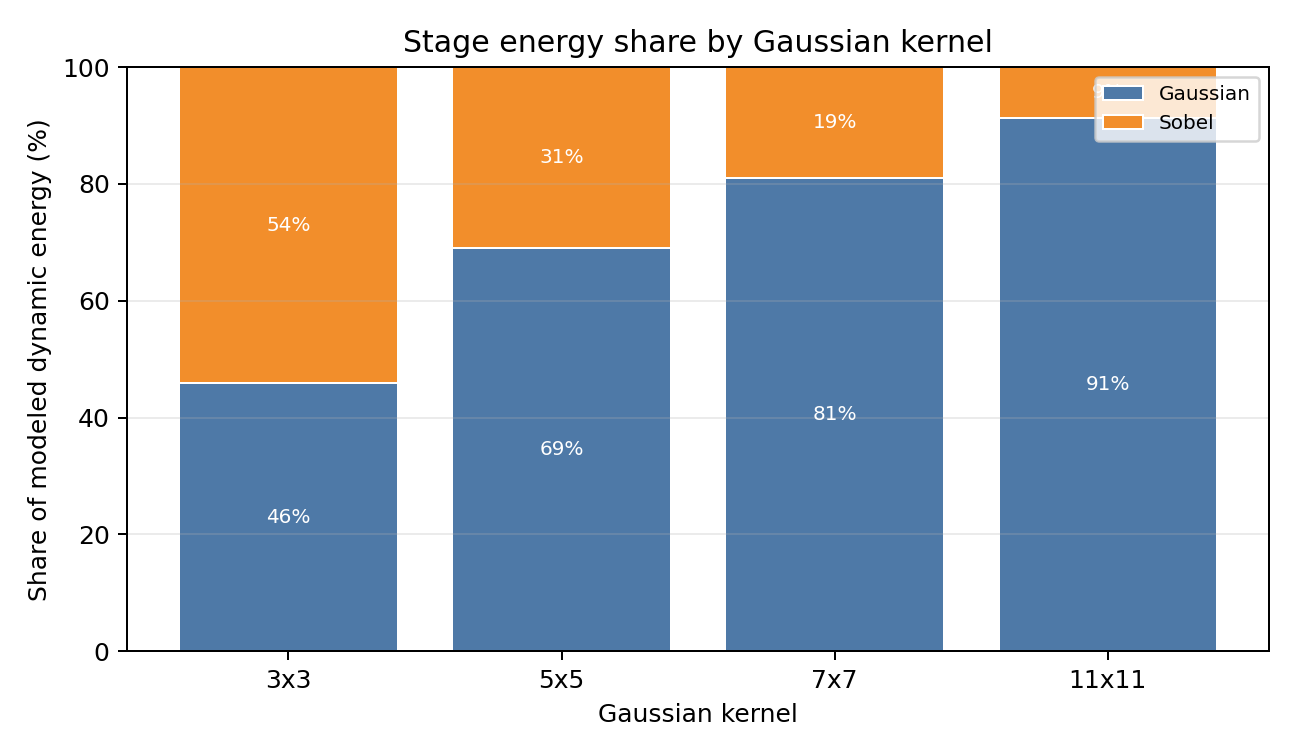
\includegraphics[width=0.9\textwidth]{stage_share_by_kernel.png}
\caption{Gaussian and Sobel energy shares for the selected 1080p designs.}
\label{fig:stage-share}
\end{figure}

\section{Component Energy Split}

Figure~\ref{fig:component-split} shows the modeled dynamic energy split across MAC, SRAM, and DRAM actions for the selected 1080p designs. The conclusion is intentionally scoped to this action-count model.

\begin{figure}[H]
\centering
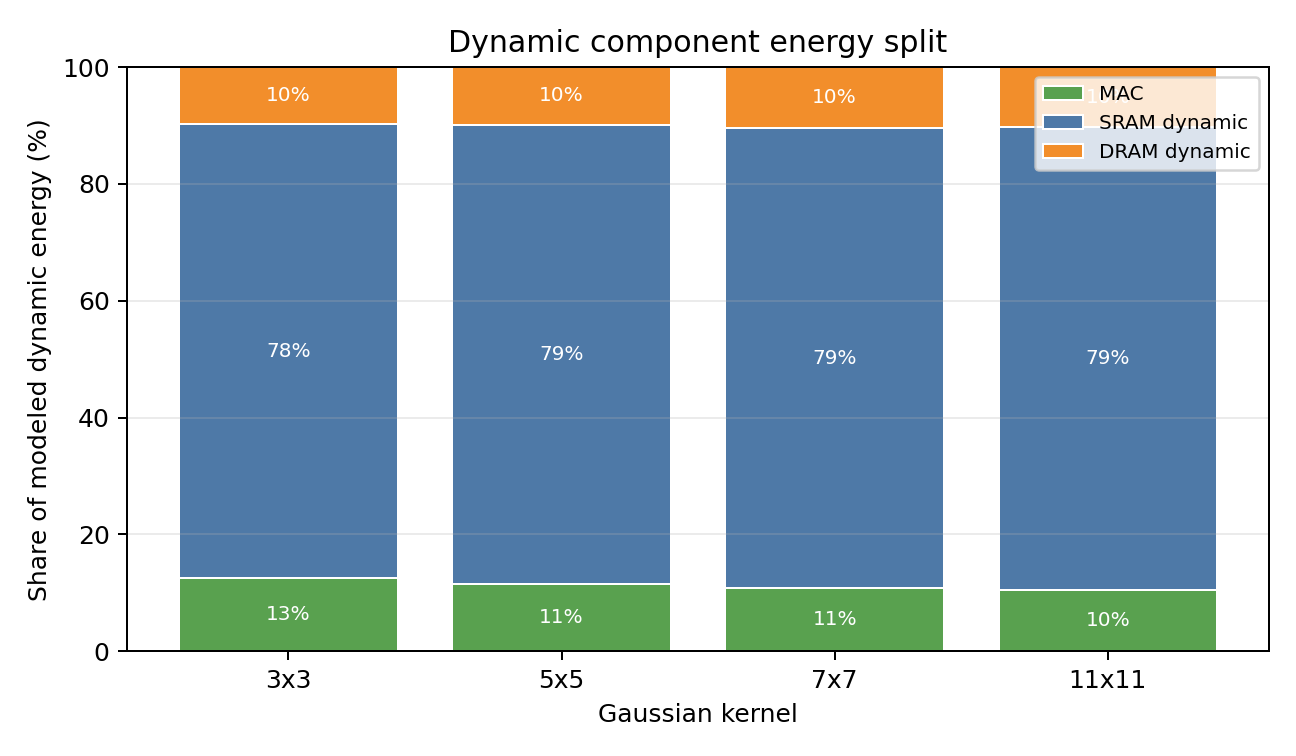
\includegraphics[width=0.9\textwidth]{component_energy_split.png}
\caption{Modeled component energy split for the selected 1080p designs.}
\label{fig:component-split}
\end{figure}

\end{document}
